\section{Forums}

The forums feature will be examined based on a framework to determine how well the implemented feature has achieved its intended purpose and its functionality.

The feature analysis includes three sections:

\begin{enumerate}
    \item \textbf{Functional Requirements} - does the forum component meet the functional requirements defined in the project approach?
    \item \textbf{Non-Functional Requirements} - does the forum component meet the non-functional requirements defined in the project approach?
    \item \textbf{Usability Tests} - what do potential users of the system think about the forums and how could it be improved?
\end{enumerate}

This section will also contain a reflection on how well milestones were met compared to the timelines set at the start of this project, as well as the challenges faced throughout this project.

\subsection{Functional Requirements}
The functional requirements of the forums are evaluated based on whether or not they were implemented in the system.
A requirement is considered complete if most or all of its acceptance criteria have been met.
The priority of the requirement has also been taken into consideration.
If a "Must Have" criteria has not been completed, then the requirement also cannot be considered completed.
Requirements and criteria marked as "Won't Have" are not considered in this evaluation.

Below is the list of functional requirements and their acceptance criteria, each marked with their status of completion.

\begin{enumerate}
    \item Users can view a list of forum posts (Completed)
\end{enumerate}
\begin{itemize}
    \setlength{\itemindent}{1.5em}
    \item Users can see all forum posts in a table (Completed)
    \item Users can see all pinned posts in a separate table (Completed)
\end{itemize}

\begin{enumerate}
    \setcounter{enumi}{1}
    \item Users can clearly see which posts have been read and actioned (Completed)
\end{enumerate}
\begin{itemize}
    \setlength{\itemindent}{1.5em}
    \item Users can easily find answered posts (Completed)
    \item Users can sort posts by number of replies or comments (Completed)
    \item Users can see which posts have been endorsed (Completed)
\end{itemize}

\begin{enumerate}
    \setcounter{enumi}{2}
    \item Users can add a post to the forum (Completed)
\end{enumerate}
\begin{itemize}
    \setlength{\itemindent}{1.5em}
    \item Users can add a post with a title and description (Completed)
    \item Users can format their post description (Completed)
    \item Users can optionally attach files (Partially Completed)
    \item Users can optionally attach tags (Completed)
    \item Users can optionally attach links (Completed)
\end{itemize}

\begin{enumerate}
    \setcounter{enumi}{3}
    \item Users are able to search for a forum post (Completed)
\end{enumerate}
\begin{itemize}
    \setlength{\itemindent}{1.5em}
    \item Users can search a post's description or title (Completed)
\end{itemize}

\begin{enumerate}
    \setcounter{enumi}{4}
    \item Users can filter through forum posts (Completed)
\end{enumerate}
\begin{itemize}
    \setlength{\itemindent}{1.5em}
    \item Users can filter forum posts using pre-defined tags (Completed)
    \item Users can filter posts by those linked to announcements (Completed)
    \item Users can filter posts by those that are answered (Completed)
    \item Users can filter posts by those that are unanswered (Completed)
    \item Users can filter posts by those that are endorsed (Completed)
\end{itemize}

\begin{enumerate}
    \setcounter{enumi}{5}
    \item Users are able to sort the forum posts (Completed)
\end{enumerate}
\begin{itemize}
    \setlength{\itemindent}{1.5em}
    \item Users can sort forum posts by different headings in the post table (Completed)
\end{itemize}

\begin{enumerate}
    \setcounter{enumi}{6}
    \item Users can view the individual post details for a chosen post (Completed)
\end{enumerate}
\begin{itemize}
    \setlength{\itemindent}{1.5em}
    \item Users can navigate to a post page for an individual post (Completed)
    \item Users can easily see the post title, description, tags, author and data created (Completed)
    \item Users can see all the responses to the post (Completed)
    \item Users can see all the comments on the post (Completed)
\end{itemize}

\begin{enumerate}
    \setcounter{enumi}{7}
    \item Users can share a forum post with others (Partially Completed)
\end{enumerate}
\begin{itemize}
    \setlength{\itemindent}{1.5em}
    \item Users can copy a link to a forum post (Completed)
    \item Users can directly share a forum post to other platforms (Not Completed)
\end{itemize}

\begin{enumerate}
    \setcounter{enumi}{8}
    \item Users can upvote a forum post (Completed)
\end{enumerate}
\begin{itemize}
    \setlength{\itemindent}{1.5em}
    \item Users can upvote a post on the forum overview page (Completed)
    \item Users can upvote a post on the forum post page (Completed)
    \item Users can see the number of upvotes a post has (Completed)
\end{itemize}

\begin{enumerate}
    \setcounter{enumi}{9}
    \item Users can edit their post (Completed)
\end{enumerate}
\begin{itemize}
    \setlength{\itemindent}{1.5em}
    \item Users can edit a post after it has been posted (Completed)
\end{itemize}

\begin{enumerate}
    \setcounter{enumi}{10}
    \item User can delete their post (Completed)
\end{enumerate}
\begin{itemize}
    \setlength{\itemindent}{1.5em}
    \item Users can delete a post after it has been posted (Completed)
\end{itemize}

\begin{enumerate}
    \setcounter{enumi}{11}
    \item Users can comment on a post (Completed)
\end{enumerate}
\begin{itemize}
    \setlength{\itemindent}{1.5em}
    \item Users can leave a comment on a forum post (Completed)
    \item Users can format their comment (Completed)
    \item Users can edit their comment after it has been posted (Completed)
    \item Users can delete their comment after it has been posted (Completed)
\end{itemize}

\begin{enumerate}
    \setcounter{enumi}{12}
    \item Staff can manage the tags for the topic group (Completed)
\end{enumerate}
\begin{itemize}
    \setlength{\itemindent}{1.5em}
    \item Staff can add new tags (Completed)
    \item Staff can remove tags (Completed)
    \item Staff are unable to create duplicate tags (Completed)
    \item Students are unable to create tags (Completed)
\end{itemize}

\begin{enumerate}
    \setcounter{enumi}{13}
    \item Staff are able to pin posts to the top of the forums (Completed)
\end{enumerate}
\begin{itemize}
    \setlength{\itemindent}{1.5em}
    \item Staff can pin posts to the top of the forums (Completed)
    \item Staff can unpin posts to the top of the forums (Completed)
    \item Staff are unable to pin and unpin posts (Completed)
\end{itemize}

\begin{enumerate}
    \setcounter{enumi}{14}
    \item Staff can reply to a forum post (Completed)
\end{enumerate}
\begin{itemize}
    \setlength{\itemindent}{1.5em}
    \item Users can leave a reply on a forum post (Completed)
    \item Users can format their reply (Completed)
    \item Users can edit their reply after it has been posted (Completed)
    \item Users can delete their reply after it has been posted (Completed)
\end{itemize}

\begin{enumerate}
    \setcounter{enumi}{15}
    \item Staff can endorse a post or comment (Completed)
\end{enumerate}
\begin{itemize}
    \setlength{\itemindent}{1.5em}
    \item Staff can endorse a post (Completed)
    \item Staff can unendorse a post (Completed)
    \item Staff can endorse a comment (Completed)
    \item Staff can unendorse a comment (Completed)
\end{itemize}

\begin{enumerate}
    \setcounter{enumi}{16}
    \item Staff can directly link or embed materials to the forum post (Partially Completed)
\end{enumerate}
\begin{itemize}
    \setlength{\itemindent}{1.5em}
    \item Staff can add a direct link to a reply (Completed)
    \item Staff can embed course materials in a reply (Not Completed)
\end{itemize}

In total, 15 out of the 17 functional requirements were completed.
The remaining two functional requirements were only partially completed.
Each of these functional requirements had one acceptance criteria that was not implemented however, both of these were lower priority tasks.
Overall, all of the high and mid priority requirements were implemented into the system.

Below is a list of incomplete requirements and acceptance criteria, and the reason behind why they were not completed.

\subsubsection{Users can share a forum post with others}

\textit{Users can directly share a forum post to other platforms (Could have)}

The original idea was that the share button on individual posts would provide users with various platforms, like Facebook Messenger and WhatsApp, in which they could select to send a direct link to the forum post to.
As this was a lower priority task, time constraints meant that it was unable to be completed on time.
Furthermore, since this functionality could be achieved by using the copy link to clipboard button that was built early in the implementation process and pasting the link to share it,
it was decided that the focus should be shifted to ensure higher priority tasks are completed instead.

\subsubsection{Staff can directly link or embed materials to the forum post}

\textit{Staff can embed course materials in a reply (Could have)}

The ability for staff to directly embed course materials into their reply to a forum post was a low priority feature that would've been nice to have.
This would've allowed staff to easily provide students who are asking for help with references and materials that could assist them.
Similar to the previous requirement, there was not enough time to build this feature and since staff already had the option to include a link to resources in their reply, this criteria was considered unnecessary.

\subsubsection{Users can add a post to the forum}

\textit{Users can optionally attach files (Should have)}

While this requirement has been marked complete, it is important to note that the current state of the forums only allows for images to be attached to posts.
This criteria has been marked as partially complete as ideally, documents and videos should be able to be attached as well.
This was unable to be done, however, due to time constraints and lack of knowledge in handling these file types.
However, since a user can still add a new post, and screenshots are the most popular type of attachment in forums, this overall requirement has been marked as completed.

\subsection{Non-functional Requirements}
This section contains an evaluation of how performant and accessible the forum component is.

Using Google Lighthouse, tests were run and the forum component was given a score out of 100 for performance and accessibility.
Google Lighthouse also produced a report with more details on ways in which the forums could be improved to produce a higher score.

\subsubsection{Performance}

\begin{figure}[h!]
    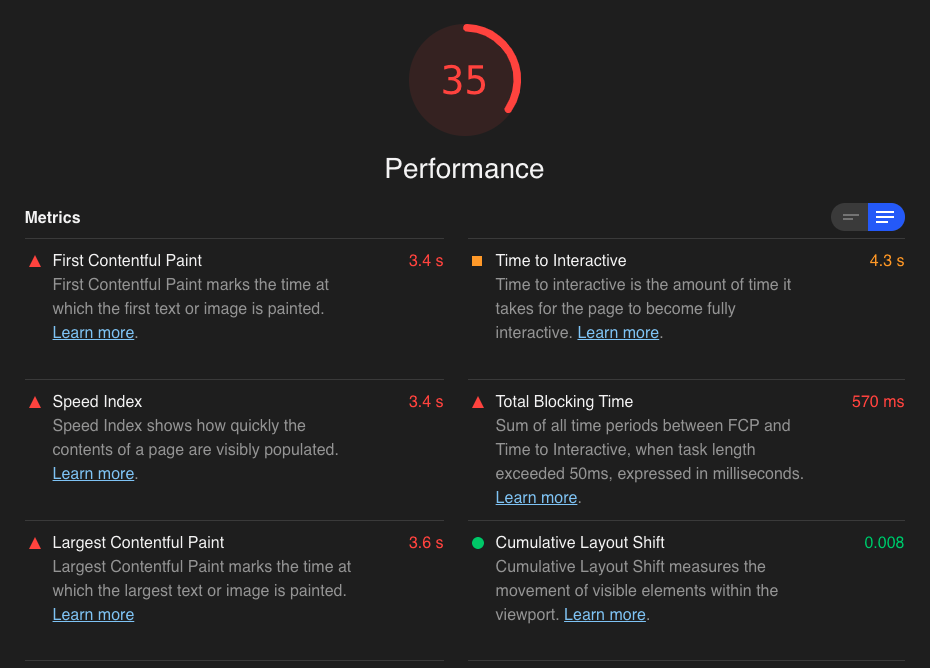
\includegraphics[scale=0.3]{forums-analysis-performance-overview-page.png}
    \centering
    \caption{Performance Report for Forums Overview Page}
\end{figure}

\begin{figure}[h!]
    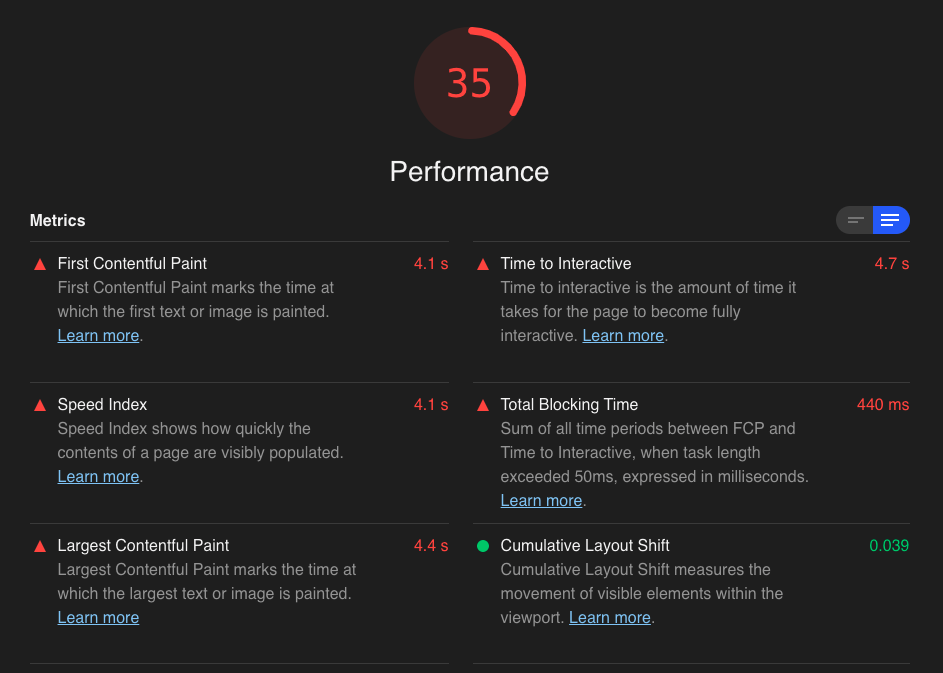
\includegraphics[scale=0.3]{forums-analysis-performance-post-page.png}
    \centering
    \caption{Performance Report for Forums Post Page}
\end{figure}

As seen from the figures above, the performance score for the forums are quite low, with a 35 out of 100 for both the overview and post pages.
Compared to the standards set by high-performing websites, the metrics measured show that the contents of the forum pages are slow to render and become interactive.
For a user with reasonable internet speeds, the slower renders would not be too noticeable.
The performance issues would mainly become a problem for users who have slow or throttled internet connections.
Despite this, performance is still an important factor when building a website and should definitely be improved in future iterations of the forum.
Refactoring the backend API and database to have a heavier focus on performance would be required to achieve this.
The report also suggests that reducing the amount of unused JavaScript could significantly reduce the load times.
This should definitely be addressed in future iterations.

On a positive note, the report shows that the forums pass the "Cumulative Layout Shift" metric.
This means that once the page has loaded, there is very minimal movement within the viewport of the user.
This is vital as it reduces the likelihood of misclicks for users.

\subsubsection{Accessibility}

\begin{figure}[h!]
    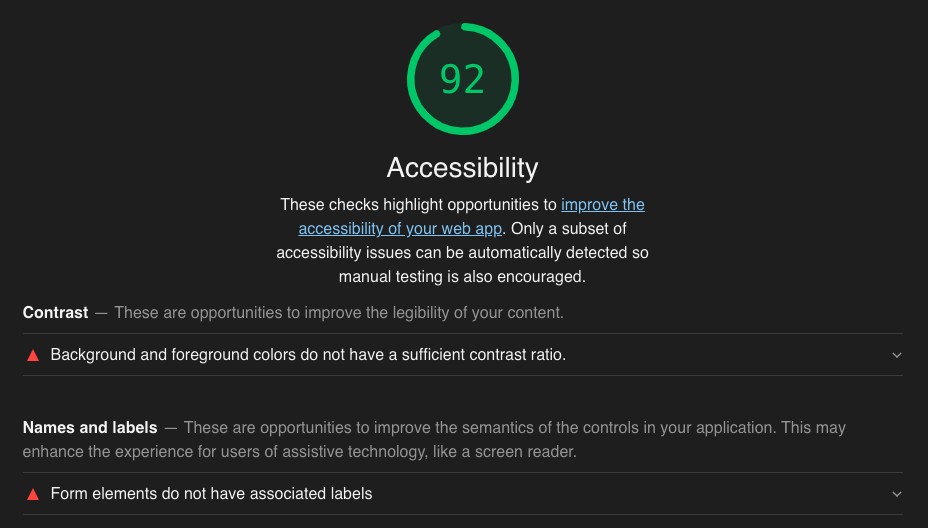
\includegraphics[scale=0.3]{forums-analysis-accessibility-overview-page.png}
    \centering
    \caption{Accessibility Report for Forums Overview Page}
\end{figure}

\begin{figure}[h!]
    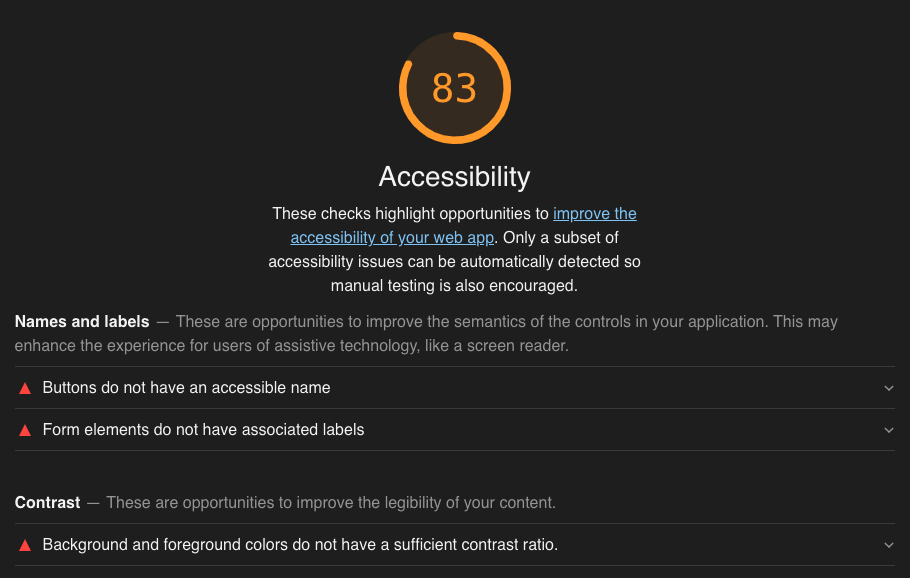
\includegraphics[scale=0.3]{forums-analysis-accessibility-post-page.png}
    \centering
    \caption{Accessibility Report for Forums Post Page}
\end{figure}

As seen from the figures above, the accessibility score for the forums was relatively high, with a 93 out of 100 for the overview page and a 83 out of 100 for the post pages.
A high accessibility score is essential for ensuring that all users, including those with disabilities, are able to use the system.
The score received for the forums is most likely due to the use of the Chakra-UI library which automatically applies a lot of the tags required for accessibility.
Even though these scores are quite high, the report suggests some easy improvements that can be made in future iterations to further improve the accessibility of the site.

Some of the colours used on both the overview and post pages do not have enough contrast with the background.
This means that people who are visually impaired may have trouble reading the words.
Since the background colour of the forums is white, making all the text darker on both pages would easily solve this problem.

A screenreader is a popular device for some people with disabilities as it can read out the components and text on a page.
As a result, it is important that all images, forms and buttons have alternative text that describes its purpose that can be read out by the device.
The report shows that on the post page, some of the buttons do not contain this alternative text.
In order to ensure that the button can be read out to users, an accessible name should be added to these buttons.
Labels should also be added to each of the input fields on the page, including those in the "Add Post" modal and in the responses and comments section of the post page.

\subsection{Usability Testing}

Simple tests were run with tutors and students to evaluate the usability of the forums component and receive feedback on ways in which the system could be improved.

\subsubsection{Audience}

In order to get a wholistic understanding of the usability of the system, participants from various fields were used to test the student's perspective of the forums component.
This is to test that the forums are appropriate for use in all types of courses. These fields included:

\begin{itemize}
    \item Engineering;
    \item Medicine;
    \item Science; and,
    \item Art and Design.
\end{itemize}

\subsubsection{Student's Perspective}

To test the forums from a student's perspective, student participants were first asked to look at the overview and post page and provide their initial thoughts.

For the forum overview page, most participants stated that on first look, they liked the way in which the posts were laid out.
They mentioned that the layout was pretty straight forward and easy to understand.
They also liked that the pinned posts were separated and located at the top of the page.

Some users, however, found that the page looked quite cluttered.
This was mainly seen in the search and filter areas at the top of the page.
This could be improved by making the search and filter areas collapsible so that students can hide them from view when not being used.
They also mentioned that the indentation on the left of the post table looked weird and was a waste of horizontal space.
When viewing the overview page from a staff perspective, this would be where the pin icon shows however this is not the case for students since they are unable to pin posts themselves.
The indentation could easily be fixed by removing the spacing or by showing the pin buttons but not making them clickable for students.

For the forum post page, all participants were initially confused by the responses and comments section.
They were unable to understand, just from looking at the page, why there were two separate sections.
When looking at a post that has some comments and replies, this confusion was cleared up a bit for some participants.
Some users were also confused by how the comments were displayed, and were unsure if the input field was for creating a new comment or to reply to the comment above.
They suggested adding placeholder text to the input field to make this clearer.

The student participants were then given various scenarios to test out different features of the forums.
For each of the scenarios, the students were asked to rate the process required to complete the task out of five, one being difficult and five being simple.

The first scenario asked the students to add a new post with a tag to the forums.
All participants found this process very simple and intuitive, giving the process a five out of five.
Participants found that it was easy to work out how to add a post due to the large call-to-action on the overview page.
They also liked that the button opened up a modal instead of making them navigate to a different page.
One participant suggested moving the tag selection to the top of the "Add Post" modal since it is easy to miss when it is at the bottom of the form.
This is something that will definitely be implemented in future iterations of this project.
Additionally, some students noticed and interacted with the edit button on the newly created post.
The main feedback that arose from this was that students would like to also be able to edit the title and tags for the post.

The second scenario required participants to filter the posts by a specific tag.
All participants found this process simple, giving it a five out of five for usability.
Some students used the dropdown menu to find the tag to filter by while others typed the tag name into the filter bar.
This shows that having both options is useful to users and it isn't redundant to have both.
Some users liked the fact that the filter displayed at the top of the page and wasn't hidden away on the side or in a menu, while others thought it cluttered up the overview page a bit.
Due to the way it was built, the filter does not persist between pages meaning that if a user filters by a tag and then goes through each of the results, they would have to re-filter the posts each time they return to the overview page.
This frustrated some participants as they expect the filter to remain when they navigate back from a post.

Participants were then asked to find a specific post and leave a reply.
In order to complete this task, some participants used the search bar, some used the sort functionality in the table and some just scrolled until they found the post.
This proves that users interact with the forums in different ways and shows that none of this functionality is useless.
Despite the method they used to find the post, all users gave this process a five out of five.
All participants also found it very easy to leave a comment and didn't have much feedback for that process.

Participants were also asked to edit their previous comment.
They all gave this process a five out of five for usability, with the size and positioning of the buttons making it easy to work out how to complete this process.
The only feedback received for this was that the participant expected the timestamp on the comment to be updated to reflect when they made the change.

Participants also found that it was extremely easy to upvote a post, with them all successfully completing the scenario and giving it a five out of five.
They appreciated the fact that they didn't have to click into a post to upvote it if they didn't want to, they could just upvote it from the overview page.
For this scenario, the participants were also asked about how they would rate the usefulness of this feature.
This was to get an understanding of whether or not the feature would actually be beneficial to users.
Pretty much all of the participants said that they personally would not upvote a post themselves however, they would definitely use the number of upvotes a post has to determine which ones were worth looking at.
As a result, on average, they gave the upvoting feature a 4.5 out of five in terms of usefulness.

Finally, the students were asked to share a post.
Most users were easily able to complete this task but some were confused about the icon on the share button and expected it to have a different functionality to sharing.
One user also didn't notice there was a share button and instead, copied the url from the url bar of the browser.
As a result, this process was given an average score of 4.5 out of five for usability.
When asked about the usefulness of this feature, most participants were unsure if it provided much value to the system since the url could just be copied from the browser.
They suggested that implementing the ability to share posts to specific platforms would make it more useful.
This is a feature that was planned however, was not achieved due to time constraints.

Overall, all student participants found that the system was easy and intuitive to use.
Most enjoyed the layout and design however, there is still improvements that could be made to please more users.

\subsubsection{Staff's Perspective}

Due to having limited time with the staff members, the usability tests for the staff-only features of the forum mainly consisted of showing the participants the overview and post pages and letting them interact with it whilst providing their thoughts and feedback.

The feedback for the forum overview page was mainly positive from all participants.
Most participants liked the fact that they could pin posts to the top, and mentioned that it was a feature that they would definitely use.
Some participants commented on the pinned posts also showing in the list of all posts and while they personally did not like this concept, they said that it didn't hinder their understanding of which posts were and weren't pinned.

There were some mixed reviews on upvotes with some participants saying that they liked the feature and would definitely use it to work out which posts require their attention first.
Others said that they prefer to just scroll and answer posts chronologically and therefore, wouldn't use the feature.

Some features that aren't included in the forums that participants said they would like to see included a "new" status on forum posts that they haven't seen yet.
They said that this would be the most useful in working out which posts to look at first.
Participants also suggested having a way to identify if a post on the overview page had been replied to by them or a different staff member.
However, they also noted that while this would be a nice feature, they preferred the existing, clean interface of the post tables compared to one with too many columns.

When it comes to tags, some participants liked the feature while some were impartial to it.
Those who liked the tags thought that it was a good way to categorise and group posts together.
Some participants, however, thought tags may be unnecessary if the search functionality of the forums is good enough.
They were also concerned about whether or not students would actually use the tags, and whether they would be used correctly.

Like the student participants, the staff were also initially confused about the difference between responses and comments.
This issue could potentially be fixed by renaming the responses section to "Official Responses", or by adding a description of what each section means below the title.

Participants also had mixed feelings about endorsing posts and comments.
Some mentioned that it felt too easy to endorse a post and suggested adding a confirmation message to ensure that the staff member hasn't misclicked the button.
Others were just unsure about how endorsing could be helpful to them however, once it was explained further, they were able to see the value of the feature.
This shows that there needs to be more explanation around what it means to endorse a post and how this can benefit the user.
This could be done by adding a tutorial tooltip to the endorse button when it is first clicked by the user.

Overall, the staff participants were happy with the forums and liked all the functionality it provided.

\subsection{Timeline}

Throughout the duration of this project, many of the originally planned tasks were able to be completed ahead of schedule.
This allowed for additional features like endorsed posts, enhanced filter and upvoting, to also be implemented.
Overall, majority of the important features were completed with enough time to conduct sufficient analysis of the system.

\subsection{Challenges}

Most of the challenges faced throughout this project occurred when working with third-party packages and libraries.

The initial rich-text editor package for React was quite difficult to work with as there was poor documentation and plugins had to be added to handle some functionality.
For example, one of the requirements for this feature was that users could embed links in their forum posts however, the original editor needed a plugin to make this possible.
The lack of documentation made it difficult to get these plugins installed and working as expected.
As a result, a different editor that had these functionalities already built in was used instead.

Another package that was difficult to work with was \texttt{react-table}.
Some of the columns in the table, like the upvote column and the pin column, displayed elements other than just text.
At first, it was difficult to work out how to achieve this however, researching the issue revealed documentation that explained how to display custom elements in the body of the table.

While most of the milestones for the forums component were able to be completed on time, there were some features that couldn't be fully implemented until close to the end of the development process due to dependencies on other LMS features.
This meant that some of the analysis and evaluation processes had to also be delayed.
This, however, is a challenge typically faced when developing a large system in parallel and was able to be overcome through open communication and discussion with other team members.
Despite this, all the main requirements for the forums were eventually able to be completed before the due date.

